\section{DTW: Dynamic Time Warping}
Il \textbf{Dynamic Time Warping} (DTW)\cite{dtw}è un algoritmo per misurare la similarità tra due TS, calcolandone il match ottimale.\\
\\
A differenza delle classiche funzioni di distanza, come quella Euclidea o la Manhattan, essa effettua un confronto di tipo \textbf{elastico} (non-lineare) tra i punti delle due TS a confronto: Esse non sono confrontate 1-a-1, matchando l'$i$-esimo punto della TS A con l'$i$-esimo punto della TS B, bensì 1-a-n, matchando un punto della TS A con uno o più punti della TS B.\\
Il confronto tra due punti matchati avviene sempre con una metrica classica, come quella Euclidea. Tutte le singole distanze tra i punti sono conservate in una \textbf{matrice di distanza}.\\
\\
Siano A e B due TS a confronto, vengono imposti i seguenti vincoli nel clacolo del DTW:
\begin{itemize}
	\item Un punto di una TS può essere matchato con uno o più punti dell'altra TS;
	\item Il match tra due punti può avviene se e solo se le due TS hanno la stessa monotonia nei rispettivi punti;
	\item Il primo punto della TS A è matchato con il primo della TS B;
	\item L'ultimo punto della TS A è matchato con l'ultimo della TS B; 
\end{itemize}
\begin{figure}[H]
	\centering
	\begin{subfigure}{.5\textwidth}
		\centering
		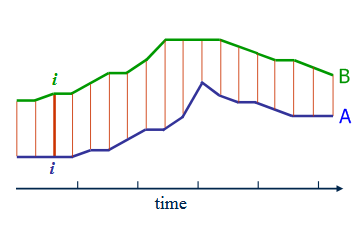
\includegraphics[width=.9\linewidth]{euclidean.png}
		\caption{Distanza Euclidea (lineare)}
		\label{fig:distance_euclidean}
	\end{subfigure}%
	\begin{subfigure}{.5\textwidth}
		\centering
		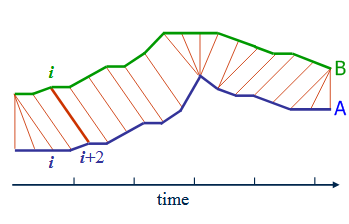
\includegraphics[width=.9\linewidth]{dtw.png}
		\caption{DTW (elastica)}
		\label{fig:distance_dtw}
	\end{subfigure}
	\caption{Confronto tra distanza Euclidea e DTW}
	\label{fig:distance}
\end{figure}
In altre parole, il DTW cerca di "allineare" al meglio le due TS, facendo in modo che entrambe proseguano con lo stesso andamento.\\
\\
La similarità del DTW produce buoni risultati per le TS che rappresentano uno stesso evento ma che sono di lunghezza differente, ad esempio quando entra in gioco uno sfasamento temporale.\\
Un individuo che pronuncia una stessa frase con lo stesso tono ma con velocità differente produrrebbe due TS molto differenti. Se esse venissero confrontate linearmente, non si potrebbe riconoscere che, difatti, l'individuo che ha prodotto tali frequenze è lo stesso. Con un confronto tramite DTW ciò viene ovviato.\\
\\
L'algoritmo compie una ricerca nella matrice di distanza, di spazio $O(mn)$, dove $m$ ed $n$ sono le lunghezze delle due TS confrontate.
Dunque, al caso pessimo e con TS molto grandi (es. centinaia di punti), il calcolo del DTW richiede un tempo impraticabile. In letteratura, perciò, sono state definite alcune implementazioni veloci, come \textit{PrunedDTW}, \textit{SparseDTW} e \textit{FastDTW}, che tentano di accelerarne il calcolo. Ciò nonostante, la tecnica resta complessa in termini di tempo e di spazio, sopratutto in caso di dataset ad alta dimensionalità.\\

\section{Confronto con k-Means di TSLearn}
Il clustering mediante l'impiego di DWT è stato realizzato sfruttando la libreria TSLearn.
Essa, infatti, come evidenziato dal nome stesso, consiste in una specializzazione del Machine Learning focalizzato sulle Time Series.
La libreria non solo offre metodi per il calcolo delle metriche proprie delle TS (\textit{DTW},\textit{Soft-DTW}, ecc.), ma anche veri e propri algoritmi di Machine Learning in una variante modificata \textit{ad hoc} per le TS, sia di tipo supervised che unsupervised (es. \textit{SVM}, \textit{TimeSeriesKMeans}).\\
\\
Proprio uno di questi algoritmi, \textit{TimeSeriesKMeans}, è stato impiegato per il nostro esperimento. 
Esso consiste in una versione modificata del noto algoritmo di clustering, abile nel calcolo dei cluster usando non solo la metrica euclidea, ma anche il DTW e il Soft-DTW.
\\
Di seguito sono riportati i risultati del clustering dei dataset in esame, con però alcune premesse:
\begin{itemize}
	\item Il Silhouette Coefficient per tutti i dataset, data l'impraticabilità di calcolo su dataset di grandi dimenioni;
	\item Non viene riportata la Relative Purity perché introdotta successivamente al calcolo di questi risultati, e una sua introduzione avrebbe richiesto un computo troppo oneroso;
	\item Per avere un riscontro diretto con le labels presente nei dataset, il numero di cluster calcolati corrisponde al numero di classi presenti nel dataset;
\end{itemize}

\subsubsection{ECG5000}
\begin{center}
	\pgfplotstabletypeset[
	col sep=comma,
	string type,
	every head row/.style={
		before row={\hline
			\multicolumn{2}{c|}{\textbf{ECG5000}} &
			\multicolumn{2}{c|}{Internal} & \multicolumn{3}{c}{External} \\
		},
		after row=\hline
	},
	every last row/.style={after row=\hline},
	]{metrics/dtw/ECG5000_dtw.csv}
	\begin{table}[H]
		\centering
		\caption{5-Means con DTW su ECG5000}
	\end{table}
\end{center}
\textbf{Gli score dell'autoencoder sono molto simili a questi}. L'autoencoder è allora riuscito ad estrarre bene le caratteristiche degli elettrocardiogrammi, come intuito dall'analisi precedente.

\subsubsection{ECG200}
\begin{center}
	\pgfplotstabletypeset[
	col sep=comma,
	string type,
	every head row/.style={
		before row={\hline
			\multicolumn{2}{c|}{\textbf{ECG200}} &
			\multicolumn{2}{c|}{Internal} & \multicolumn{3}{c}{External} \\
		},
		after row=\hline
	},
	every last row/.style={after row=\hline},
	]{metrics/dtw/ECG200_dtw.csv}
	\begin{table}[H]
		\centering
		\caption{2-Means con DTW su ECG200.}
	\end{table}
\end{center}
\textbf{Gli score dell'autoencoder con 2-Means sono migliori rispetto a questi}. La causa potrebbe essere la dimensione ridotta del dataset che non ha permesso TSLearn di operare bene.

\subsubsection{ChlorineConcentration}
\begin{center}
	\pgfplotstabletypeset[
	col sep=comma,
	string type,
	every head row/.style={
		before row={\hline
			\multicolumn{2}{c|}{\textbf{Chlorine}} &
			\multicolumn{2}{c|}{Internal} & \multicolumn{3}{c}{External} \\
		},
		after row=\hline
	},
	every last row/.style={after row=\hline},
	]{metrics/dtw/ChlorineConcentration_dtw.csv}
	\begin{table}[H]
		\centering
		\caption{3-Means con DTW su ChlorineConcentration.}
	\end{table}
\end{center}
\textbf{Gli score dell'autoencoder con 3-Means sono quasi identici a questi}. L'autoencoder è allora riuscito ad estrarre bene le caratteristiche di queste TS, cosa non colta durante l'analisi precedente.

\subsubsection{FordA}
\begin{center}
	\pgfplotstabletypeset[
	col sep=comma,
	string type,
	every head row/.style={
		before row={\hline
			\multicolumn{2}{c|}{\textbf{FordA}} &
			\multicolumn{2}{c|}{Internal} & \multicolumn{3}{c}{External} \\
		},
		after row=\hline
	},
	every last row/.style={after row=\hline},
	]{metrics/dtw/FordA_dtw.csv}
	\begin{table}[H]
		\centering
		\caption{2-Means con DTW su FordA.}
	\end{table}
\end{center}
\textbf{Tutti gli score dell'autoencoder con 2-Means sono quasi tutti peggiori}, ad eccezione del FMI, dove in entrambi i casi non è ottimale. L'autoencoder non è riuscito ad estrarre bene le caratteristiche di queste TS rumorose, cosa già dedotto dall'analisi precedente. 

\subsubsection{FordB}
\begin{center}
	\pgfplotstabletypeset[
	col sep=comma,
	string type,
	every head row/.style={
		before row={\hline
			\multicolumn{2}{c|}{\textbf{FordB}} &
			\multicolumn{2}{c|}{Internal} & \multicolumn{3}{c}{External} \\
		},
		after row=\hline
	},
	every last row/.style={after row=\hline},
	]{metrics/dtw/FordB_dtw.csv}
	\begin{table}[H]
		\centering
		\caption{2-Means con DTW su FordB.}
	\end{table}
\end{center}
\textbf{Gli score interni dell'autoencoder con 2-Means sono tutti peggiori}, mentre gli score esterni risultano abbastanza simili. Similmente a FordA, l'autoencoder non è riuscito ad estrarre bene le caratteristiche di queste TS rumorose, cosa già dedotto dall'analisi precedente. 

\subsubsection{PhalangesOutlineCorrect}
+++++TODO++++

\subsubsection{RefrigerationDevices}
\begin{center}
	\pgfplotstabletypeset[
	col sep=comma,
	string type,
	every head row/.style={
		before row={\hline
			\multicolumn{2}{c|}{\textbf{RefrigerationDevices}} &
			\multicolumn{2}{c|}{Internal} & \multicolumn{3}{c}{External} \\
		},
		after row=\hline
	},
	every last row/.style={after row=\hline},
	]{metrics/dtw/RefrigerationDevices_dtw.csv}
	\begin{table}[H]
		\centering
		\caption{3-Means con DTW su RefrigerationDevices.}
	\end{table}
\end{center}
Similmente a FordA, \textbf{Tutti gli score dell'autoencoder con 3-Means sono quasi tutti peggiori}, ad eccezione del FMI, dove in entrambi i casi non è ottimale. L'autoencoder non è riuscito ad estrarre bene le caratteristiche di queste TS rumorose, cosa già dedotto dall'analisi precedente. 

\subsubsection{TwoLeadECG}
\begin{center}
	\pgfplotstabletypeset[
	col sep=comma,
	string type,
	every head row/.style={
		before row={\hline
			\multicolumn{2}{c|}{\textbf{TwoLeadECG}} &
			\multicolumn{2}{c|}{Internal} & \multicolumn{3}{c}{External} \\
		},
		after row=\hline
	},
	every last row/.style={after row=\hline},
	]{metrics/dtw/TwoLeadECG_dtw.csv}
	\begin{table}[H]
		\centering
		\caption{2-Means con DTW su TwoLeadECG.}
	\end{table}
\end{center}
\textbf{Il DB dell'autoencoder con 2-Means è migliore}. Le restanti misure sono pressocché simili.

\subsubsection{TwoPatterns}
++++TODO++++

\section{Confronto con altre tecniche di feature extraction and selection}
Sono stati reperiti alcuni risultati di clustering sui dataset in esame attuando però altre tecniche di feature extraction and selection. Il clustering è stato fatto con k-Means con k pari al numero di classi del dataset e su un numero differente di feature estratte in modo diverso:
\begin{itemize}
	\item Tutte le feature estratte da \textbf{TSFresh};
	\item Feature rilevanti selezionate da TSFresh;
	\item Feature rilevanti selezionate dall'algoritmo \textbf{NDFS};
	\item Feature rilevanti selezionate dall'algoritmo \textbf{Lap Score}.
\end{itemize}
Degli score riportati nelle seguenti tabelle, solamente silhouette, Davies-Bouldin e purity verranno usate per il confronto.

\subsubsection{ECG5000}
\begin{figure}[H]
	\centering
	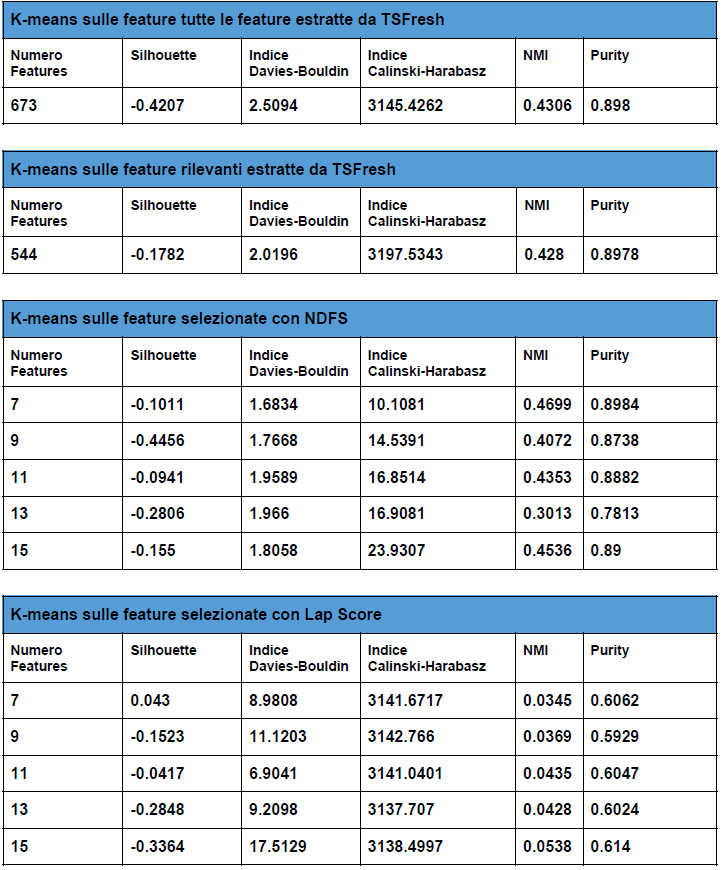
\includegraphics[width=\linewidth]{av/ecg5000_av.png}
	\caption{ECG5000 con tecniche di feature extraction and selection. TSFresh ed NDFS riportano DB e purity simili a quelli dell'autoencoder, mentre LapScore inizia a peggiorarli di molto. L'autoencoder ha migliore silhouette in ogni caso.}
	\label{fig:ecg5000_av}
\end{figure}

\subsubsection{ECG200}
\begin{figure}[H]
	\centering
	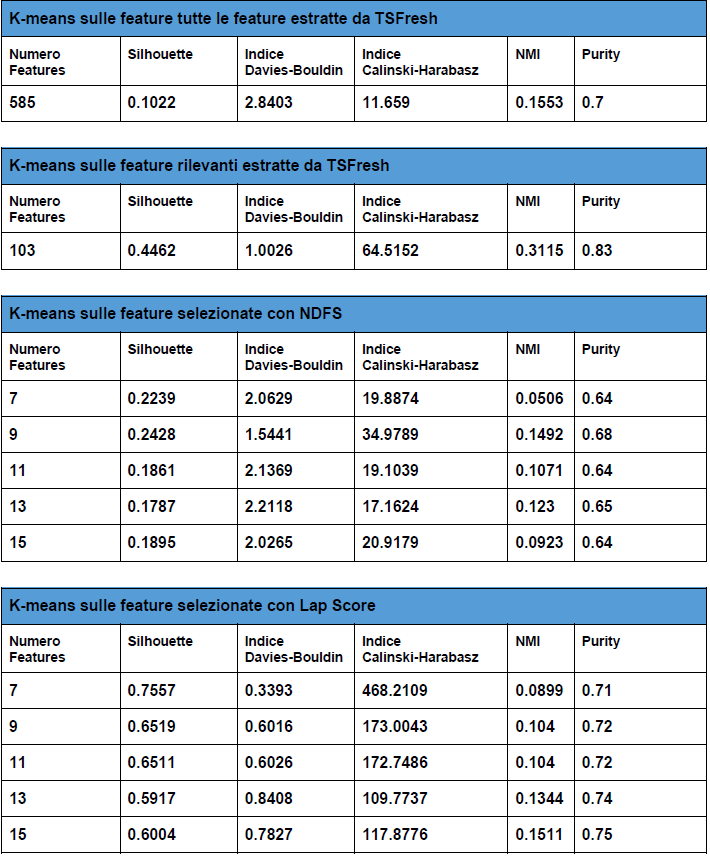
\includegraphics[width=\linewidth]{av/ecg200_av.png}
	\caption{ECG200 con tecniche di feature extraction and selection. La purity è molto simile ai risultati dell'autoencoder. La silhouette dell'autoencoder è migliore rispetto a TSFresh e NDFS, ma peggiore rispetto a Lap Score. Analogo discorso per DB, eccetto che per le feature rilevanti di TSFresh è molto simile.}
	\label{fig:ecg200_av}
\end{figure}

\subsubsection{ChlorineConcentration}
\begin{figure}[H]
	\centering
	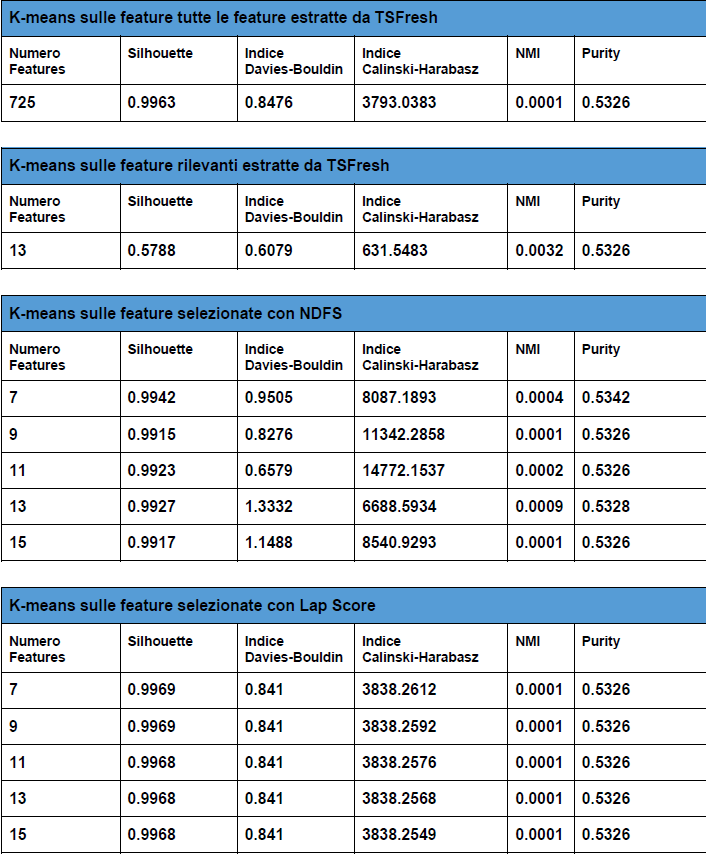
\includegraphics[width=\linewidth]{av/chlorine_av.png}
	\caption{ChlorineConcentration con tecniche di feature extraction and selection. La silhouette ritornata dall'autoencoder è peggiore, in particolar modo rispetto ad NDFS e Lap Score, mentre il DB è simile, alternando casi in cui l'autoencoder vince rispetto a qualche tecnica. La purity è pressocché indentica per tutti.}
	\label{fig:chlorine_av}
\end{figure}

\subsubsection{FordA}
\begin{figure}[H]
	\centering
	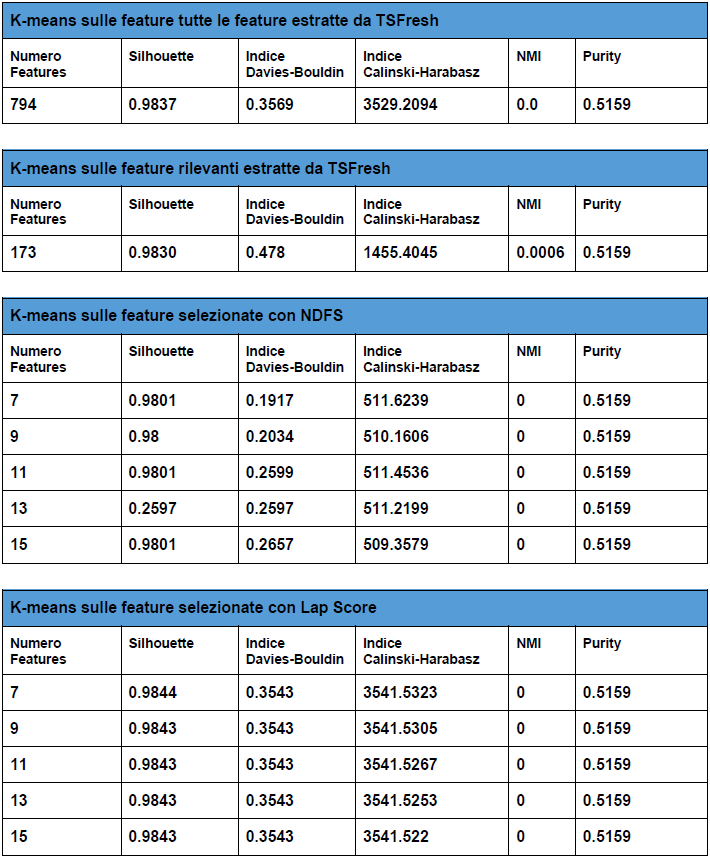
\includegraphics[width=\linewidth]{av/forda_av.png}
	\caption{FordA con tecniche di feature extraction and selection. Gli score interni ritornati dall'autoencoder sono di gran lunga peggiori in tutti i casi, mentre la purity è pressocché identica. DB è particolarmente ottimale con NDFS.}
	\label{fig:forda_av}
\end{figure}

\subsubsection{FordB}
\begin{figure}[H]
	\centering
	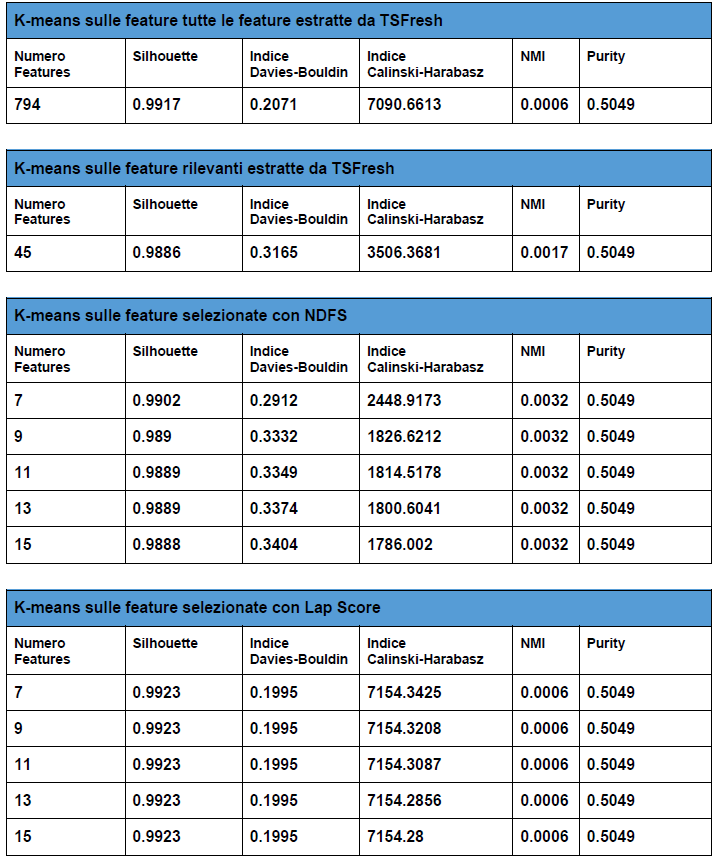
\includegraphics[width=\linewidth]{av/fordb_av.png}
	\caption{FordB con tecniche di feature extraction and selection. Come per FordA, gli score interni ritornati dall'autoencoder sono di gran lunga peggiori in tutti i casi, mentre la purity è pressocché identica. DB è particolarmente ottimale con Lap Score.}
	\label{fig:fordb_av}
\end{figure}

\subsubsection{PhalangesOutlineCorrect}
\begin{figure}[H]
	\centering
	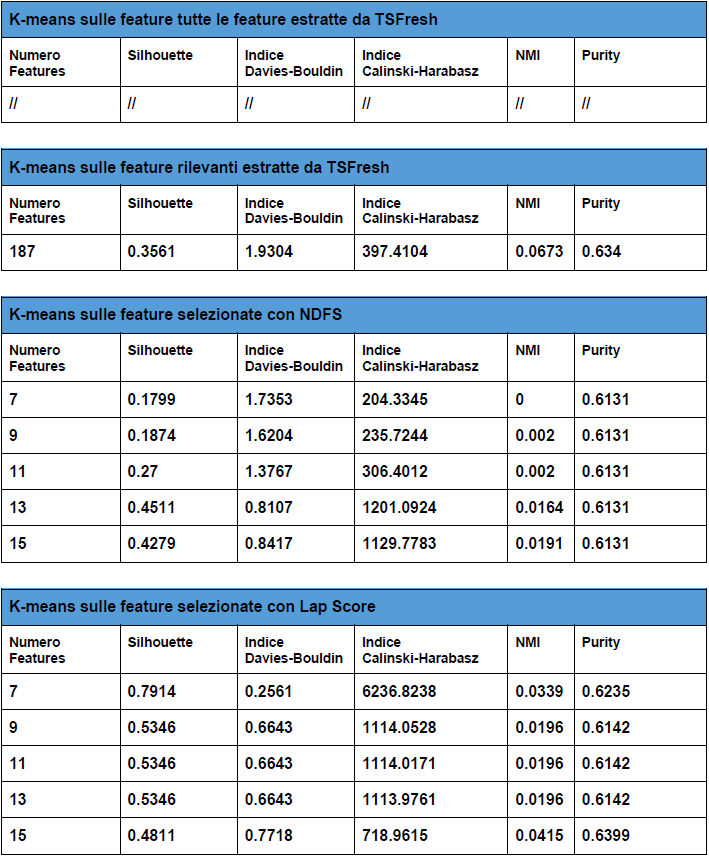
\includegraphics[width=\linewidth]{av/phalanges_av.png}
	\caption{PhalangesOutlineCorrect con tecniche di feature extraction and selection. Silhouette e DB sono variabili: qualche volta sono migliori nell'autoencoder (caso TSFresh e una parte di NDFS), altre volte è peggiore (caso Lap Score e l'altra parte di NDFS). La purity è pressocché identica in tutti i casi.}
	\label{fig:phalanges_av}
\end{figure}

\subsubsection{RefrigerationDevices}
\begin{figure}[H]
	\centering
	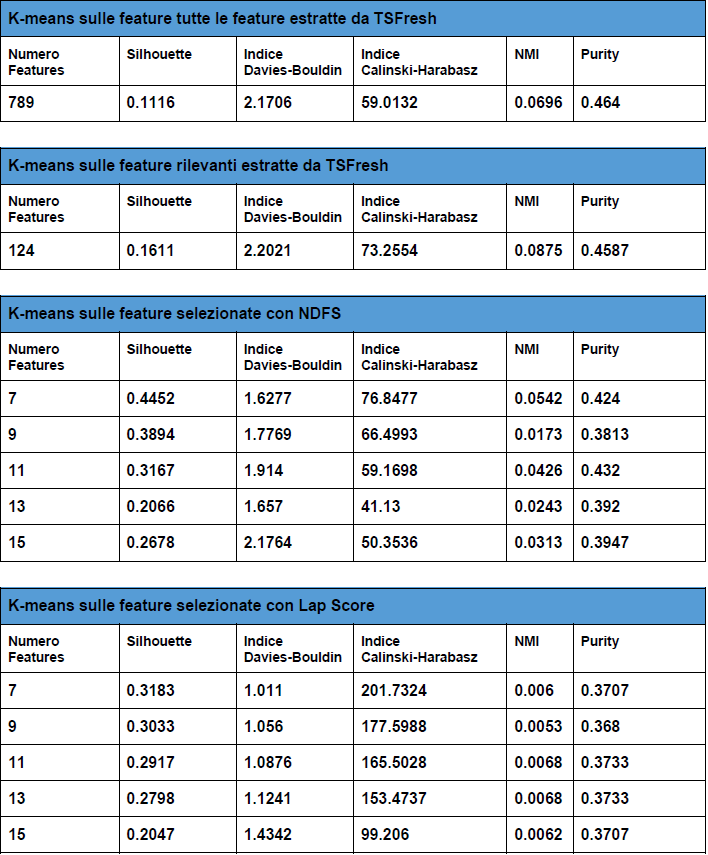
\includegraphics[width=\linewidth]{av/refrigeration_av.png}
	\caption{RefrigerationDevices con tecniche di feature extraction and selection. Con la feature selection di NDFS e Lap Score la silhouette migliora, mentre resta molto bassa con l'autoencoder o TSFresh. DB dell'autoencoder è peggiore. La purity è abbastanza simile in tutti i casi, a meno di leggere differenze.}
	\label{fig:refrigeration_av}
\end{figure}

\subsubsection{TwoLeadECG}
\begin{figure}[H]
	\centering
	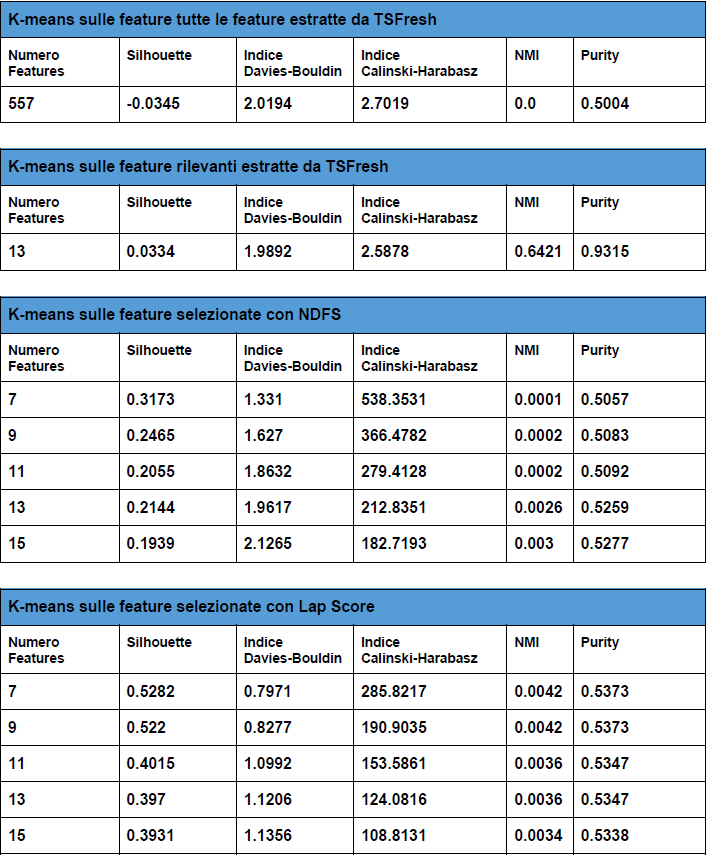
\includegraphics[width=\linewidth]{av/twoleadecg_av.png}
	\caption{TwoLeadECG con tecniche di feature extraction and selection. Silhouette e DB dell'autoencoder sono leggermente peggiori delle migliori silhouette e DB ottenuti in una delle esecuzioni di Lap Score, quindi mediamente l'autoencoder ha avuto score migliori. La purity è pressocché identica in tutti i casi eccetto il caso delle feature rilevanti di TSFresh dove è nettamente superiore.}
	\label{fig:twoleadecg_av}
\end{figure}

\subsubsection{TwoPatterns}
\begin{figure}[H]
	\centering
	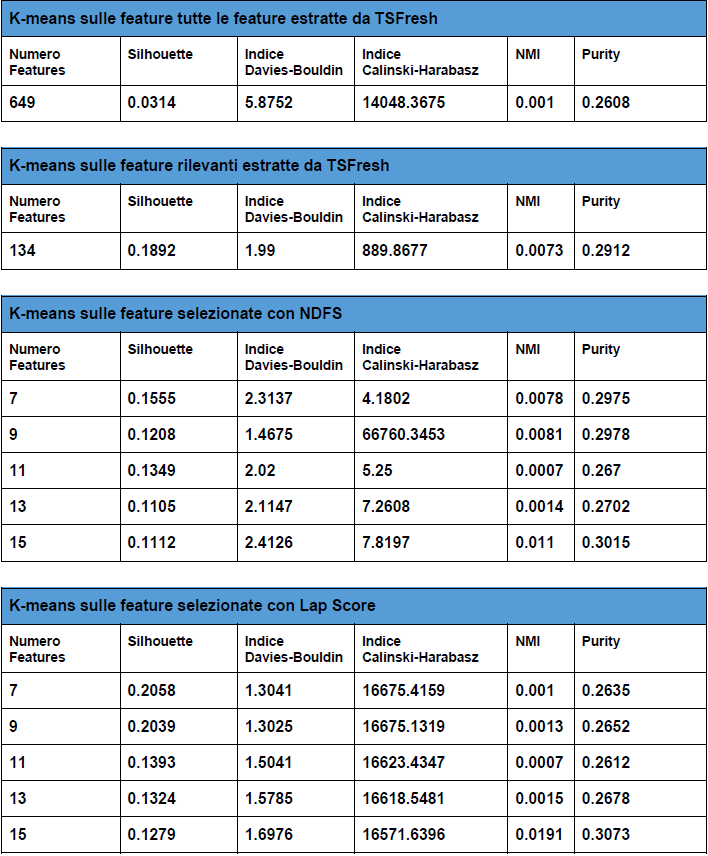
\includegraphics[width=\linewidth]{av/twopatterns_av.png}
	\caption{TwoPatterns con tecniche di feature extraction and selection. Sebbene quella dell'autoencoder sia una delle silhouette peggiori, è in generale molto bassa in tutti i casi, quindi potrebbe essere molto legato alla natura dei dati o di k-Means. Analogo ragionamento per DB. La purity è molto simile in tutti i casi, sebbene non siano ottimi valori.}
	\label{fig:twopatterns_av}
\end{figure}